\documentclass[letter, 11pt]{article}
\usepackage{fullpage}
\usepackage[margin=0.5in]{geometry}
\usepackage{graphicx}
\usepackage{caption}
\usepackage{subcaption}
\usepackage{listings}
\usepackage{amsmath}
\usepackage{float}

\begin{document}
\noindent
\large \textbf{Rahul Ghosh} \hfill \textbf{Assignment\#1}\\
\normalsize Student ID: 5476965 \hfill CSci 5561\\

\section*{HISTOGRAM OF ORIENTED GRADIENTS}
\subsection*{Method}
The given gray-scale image is differentiated along the x and y direction by convolving with the following filters:
\begin{equation*}
    filter\_x = \begin{bmatrix}
    1 & 0 & -1\\
    1 & 0 & -1\\
    1 & 0 & -1\\
    \end{bmatrix}
    and\ filter\_y = \begin{bmatrix}
    1 & 1 & 1\\
    0 & 0 & 0\\
    -1 & -1 & -1\\
    \end{bmatrix}
\end{equation*}
The gradient magnitude and direction are then calculated from the filtered images along the x and y directions. The image is divided into blocks and the gradients in each block are divided into 6 different bins according to their gradient angle. Following are the bins used in this assignment:
\begin{equation*}
    bin_1 = [\frac{11\pi}{12}, \pi)\cup[0, \frac{\pi}{12}),
    bin_2 = [\frac{\pi}{12}, \frac{3\pi}{12}),
    bin_3 = [\frac{3\pi}{12}, \frac{5\pi}{12}),
    bin_4 = [\frac{5\pi}{12}, \frac{7\pi}{12}),
    bin_5 = [\frac{7\pi}{12}, \frac{9\pi}{12}),
    bin_6 = [\frac{9\pi}{12}, \frac{11\pi}{12})
\end{equation*}
Next, to take into account the illumination and contrast, the histograms of gradients of each block is normalized using its $2\times2$ neighbors and the corresponding histograms are concatenated resulting in a 24 ($6\times4$, one for each block) length hog descriptor for each block.

To visualize, we take the sum of the magnitude for each bin and take the mid point of the bin as the angle as shown below:
\begin{equation*}
    \theta_1 = 0, \theta_2 = \frac{2\pi}{12}, \theta_3 = \frac{4\pi}{12}, \theta_4 = \frac{6\pi}{12}, \theta_5 = \frac{8\pi}{12}, \theta_6 = \frac{10\pi}{12}
\end{equation*}

The vector is plotted on the given block centre using the $quiver$ function in MATLAB. 
\subsection*{HOG Features}
\begin{figure}[!h]
\minipage{0.33\textwidth}
  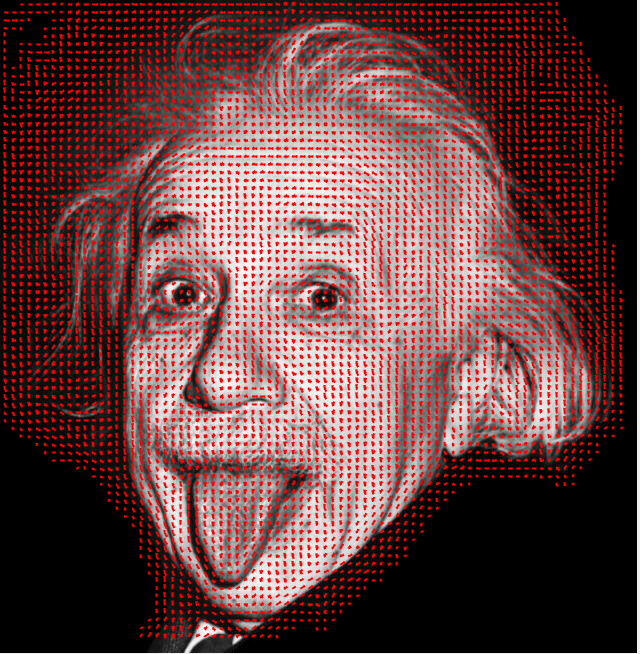
\includegraphics[width=\linewidth]{HW1/RESULT/HOG.png}
  \subcaption{HOG}\label{fig:HOG IMAGE}
\endminipage\hfill
\minipage{0.33\textwidth}
  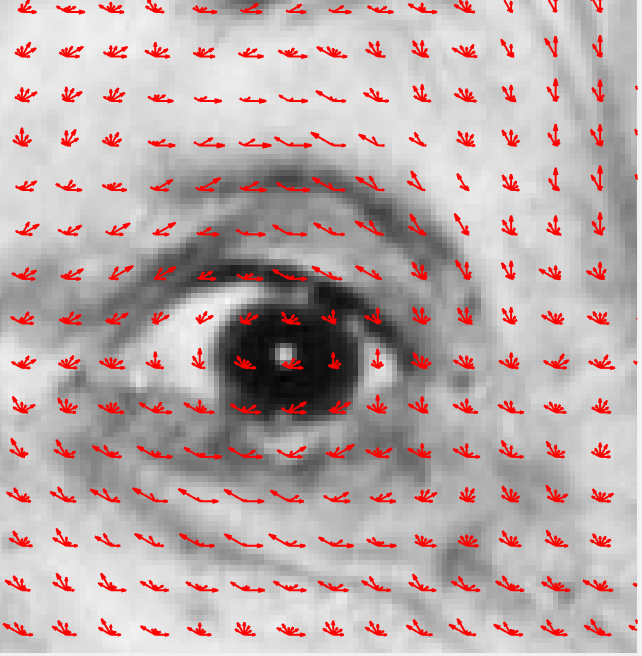
\includegraphics[width=\linewidth]{HW1/RESULT/HOG_EYE.png}
  \subcaption{HOG-EYE}
  \label{fig:HOG EYE IMAGE}
\endminipage\hfill
\minipage{0.33\textwidth}
  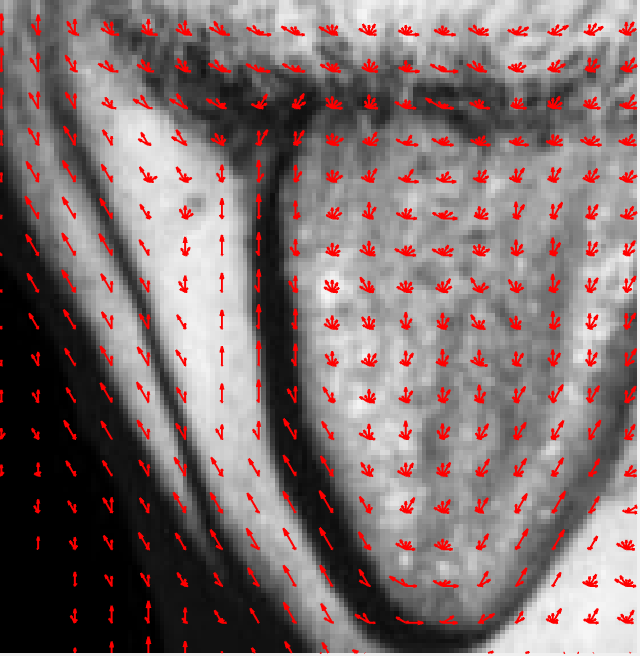
\includegraphics[width=\linewidth]{HW1/RESULT/HOG_TONGUE.png}
  \subcaption{HOG-TONGUE}
  \label{fig:HOG TONGUE IMAGE}
\endminipage\hfill
\caption{Visualizing the HOG features}
\label{fig:fig}
\end{figure}

\end{document}